\section{Experimental Evaluation}
\label{sec:eval}
The core experimental records cover already-running platform and simulator services; no Agent harness was active in the integrated runs. The full active-service snapshot was not captured, so these results describe the recorded paths rather than a frozen release. The architecture defines task-mediated and direct routes to shared dispatch, but the experiments do not establish end-to-end execution through a registered harness or equivalence between the entry paths.

Most blocks used benchmark mode, which relaxes normal timing and hold-window controls; separate production-mode guard checks are reported on their own. No cold-start deployment or physical-plant run was performed. The evaluation follows selected paths from configured mapping and write admission to process observations and exploratory Agent episodes. Because the blocks use different units—mapping requests, fixed stimuli, per-seed endpoints, a single simulated-twin execution, and Agent episodes—the counts are not pooled.

Table~\ref{tab:evidence-scope} connects each evaluation block to the question it can answer. A matching readback checks the actuator value returned by the simulator; it does not establish a process response. Conversely, an in-band process observation does not by itself establish which write caused it. The route and guard checks address pre-dispatch behavior, whereas the live-Agent episodes address whether a task reached a governed write. These distinctions determine the scope of the conclusions below.

\begin{table*}[!t]
\centering
\caption{Evaluation blocks, observational units, and limits of interpretation.}
\label{tab:evidence-scope}
\footnotesize
\setlength{\tabcolsep}{5pt}
\begin{tabularx}{\textwidth}{@{}>{\raggedright\arraybackslash}p{0.19\textwidth}>{\raggedright\arraybackslash}p{0.18\textwidth}>{\raggedright\arraybackslash}p{0.28\textwidth}X@{}}
\toprule
Block & Unit & Observation & Interpretation boundary \\
\midrule
Mapping probes & Configured request & Acceptance, rejection, and available simulated readback & Same configured limits supply inputs and checks; no physical actuation \\
Guard ablation & Fixed stimulus and technical repetition & Hypertext Transfer Protocol (HTTP) response status & One scene; benchmark mode; no readback-mismatch stimulus \\
E6 paired comparison & Scene--seed pair & Trapezoidal IAE over a fixed horizon & 11 post-pilot attempts; 9 valid pairs, 2 invalid sampling records; exploratory scripted policy versus no-write \\
Injection-twin pilot & One scripted execution & Write receipt, readback, and later process observation & No replication; incomplete raw series and runtime provenance \\
E7 Agent pilot & Episode & Task status, process value, and recorder-reported writes & Three episodes; all canceled and below band; no archived server journal \\
\bottomrule
\end{tabularx}
\end{table*}

\subsection{Configured Mapping and Integration Checks}
\label{sec:eval-mapping}
Two integrated executions each passed 77 assertions across 17 phases. These assertions provide repeated checks of the configured service path; they are not independent trials.

The two executions used seed 42, started with the platform and simulator already running, and did not activate an Agent harness. A separate preset check within the integrated film-line path configured five endpoint types and rejected nine selected negative probes. It reused the same runtime, so it is not a cold-start deployment or an independent replication of the mapping matrix.

The scene--protocol probes covered 55 writable nodes across four simulated scenes and five configured protocol variants. The variants included Transmission Control Protocol (TCP), Modbus remote terminal unit (RTU) mode, OPC UA, MQTT, and HTTP. Each node received three interior-value requests, one upper-boundary request, and four structural-range requests. All 220 admissible requests were accepted; 219 collected structural-range requests were rejected; and all 216 available readbacks matched. These probes check the consistency of configured mappings: the tested values and guards use the same configured limits. Simulator readback echoes the configured value and does not verify physical actuation. One structural request was not collected, HTTP nodes do not expose readback, and the full scene--protocol matrix remains incomplete. The excluded cast-film run and other deviations are documented in Supplementary File~S7.

\begin{table*}[!t]
\centering
\caption{Scene--protocol probes. Admissible, structural, and readback columns give accepted, rejected, and matching counts from the frozen batch; window counts are from a separate follow-up batch. Readback counts include accepted requests for which the simulator exposes an actuator value.}
\label{tab:scene-probe-results}
\footnotesize
\setlength{\tabcolsep}{3pt}
\begin{tabularx}{\textwidth}{@{}>{\raggedright\arraybackslash}p{1.55cm}r X r r r r@{}}
\toprule
Scene & Nodes & Protocols represented & Admissible & Structural & Readback & Window$^{\dagger}$ \\
\midrule
Injection & 11 & TCP 5; RTU 2; OPC UA 3; MQTT 1 & 44/44 & 44/44 & 44/44 & 22/22 \\
Wastewater & 7 & TCP 1; RTU 3; OPC UA 2; MQTT 1 & 28/28 & 28/28 & 28/28 & 14/14 \\
Annealing & 7 & TCP 3; RTU 2; OPC UA 1; MQTT 1 & 28/28 & 28/28 & 28/28 & 14/14 \\
Biaxial line & 30 & TCP 20; RTU 1; OPC UA 8; HTTP 1 & 120/120 & 119/119 & 116/116 & 60/60 \\
\bottomrule
\end{tabularx}\\
{\footnotesize $^{\dagger}$ Follow-up batch: recipe-window violations rejected / tested; counts are not pooled with the frozen batch.}
\end{table*}

\subsection{Write-Guard and Route Checks}
\label{sec:eval-ablation}
The ablation used one scene, direct API calls, a mock driver, and three deterministic repetitions per guard setting in benchmark mode. Each repetition submitted four structural-range violations and two process-window violations, as well as three legal and three boundary requests. The timed writes used for latency summaries were excluded from these counts. With all guards enabled, all six targeted process-window violations returned HTTP 400. With the process-window check removed, all six returned HTTP 200; structural violations continued to be rejected. The four structural violations were rejected in every repetition and setting; the nine legal requests per setting were accepted and the nine boundary expectations were met. These deterministic fixture counts are not independent trials or a safety rate. The archive lacks response bodies and per-request driver-call logs, so an HTTP 200 response alone does not establish driver invocation; the experiment included no readback-mismatch stimulus.

Separate scripted probes reached the expected approval and authorization branches. In the manual approval fixture, the approved request changed the simulated value from 202 to 204.8, while the rejected request left it at 216. The corresponding automatic calls did not form clean matched pairs because their labels and values did not align with those of the manual arms. No operator made the approval decisions. The probes show route handling in the tested fixture, not the effect of human approval or a general safety rate.

In a November 5 follow-up, a separate four-scene probe batch returned \texttt{RECIPE\_LIMIT\_EXCEEDED} for all 110 tested requests outside their configured recipe windows but within structural limits. The deterministic inputs and checks derive from the same configuration, so the count assesses the selected cases rather than a population failure rate. In a separate simulated injection-node fault injection, a 230-unit command produced a 251-unit readback against a 0.7-unit tolerance and was reported as \texttt{unverified}; one baseline and one recovery returned \texttt{readback-verified}. This tests one injected mismatch, not physical-device behavior. The later batch is not pooled with the frozen core results; its records and provenance limits are in Supplementary File~S7.

In a separate production-mode check, one legal baseline was accepted, and one case each was rejected for interval, step, node-range, recipe-window, and hold-window constraints. A three-case authorization probe rejected an unbound request and a cross-node request while accepting a bound write. These individual branch checks complement the benchmark-mode ablation but do not measure coverage across configurations. Full call records are listed in Supplementary File~S7.

\subsection{Fixed-Horizon Process Comparison}
\label{sec:eval-optimization}
The E6 comparison evaluated the paper's deterministic \texttt{recipe\_trial} policy (C1) against a no-write control (C0) in three simulated scenes: injection, wastewater, and annealing. The plan fixed four seeds per scene, independent fresh resets for each arm, setpoint verification, and a pre-registered initial-process-value window. Arm order was randomized within each block. The horizons were 180~s for injection and 240~s for the other scenes, with 1-s sampling. The primary outcome was trapezoidal integral absolute error (IAE); for each valid pair, $\Delta\mathrm{IAE}=\mathrm{IAE}_{C0}-\mathrm{IAE}_{C1}$, so a positive value indicates lower IAE under the scripted policy. The injection seed-43 block was designated as a pilot and is excluded from the comparison. Blocks 2--12 therefore provide 11 post-pilot attempts. A pair was valid only when both arms met the reset, initial-state, and trajectory-coverage criteria; pairs with a sampling gap greater than 5~s were retained as invalid and not replaced.

Nine of the 11 post-pilot attempts were valid, and each had a positive $\Delta\mathrm{IAE}$. The per-scene median differences were 165.165~g\,s for injection (3/3 valid pairs), 615.605~mg/L\,s for wastewater (3/4), and 8000.45~HV\,s for annealing (3/4). The valid-pair ranges were 162.535--195.169, 611.670--630.980, and 7930.200--8084.150 in the corresponding native units multiplied by seconds. The two invalid pairs were wastewater seed~45 (a 9-s gap in C0) and annealing seed~46 (a 6-s gap in C0). The separate injection pilot had $\Delta\mathrm{IAE}=163.240$~g\,s and is reported only in S7. Fig.~\ref{fig:latest-evaluation}(a) displays the nine valid paired differences and their per-scene medians. This small exploratory comparison tests one scripted policy against no-write in simulation; it is not a powered estimate, a comparison with PID, or evidence of LLM policy performance. Seeds index simulator initializations, not independent production lines.

\begin{figure*}[!t]
\centering
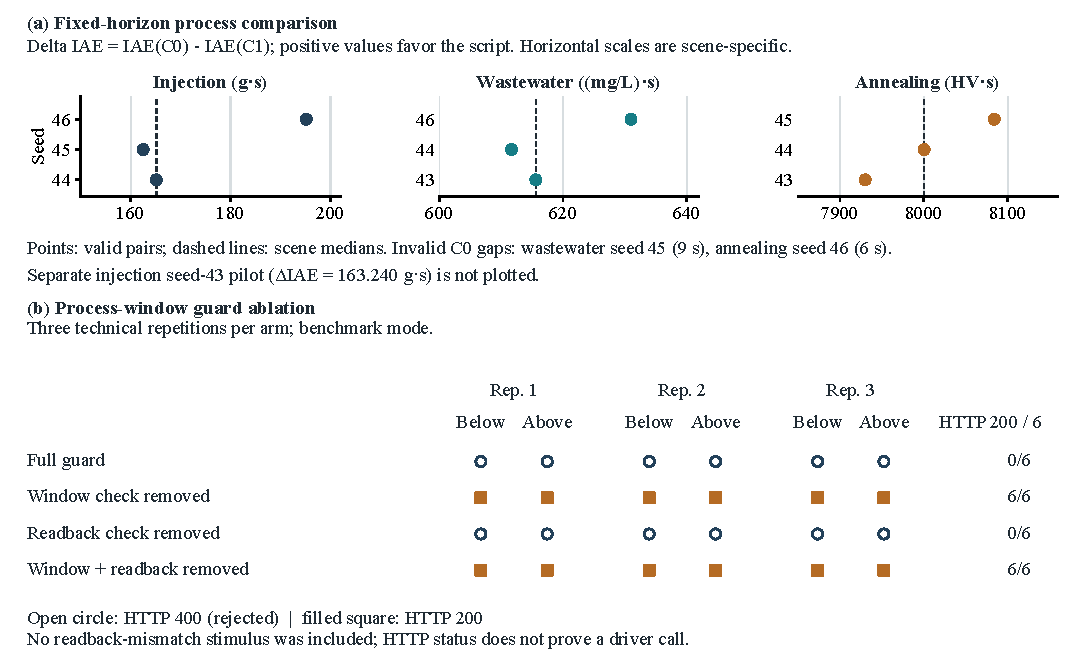
\includegraphics[width=\textwidth]{../figures/fig5.pdf}
\caption{Matched-horizon process comparison and guard-ablation responses. (a) Each point is a valid E6 scene--seed difference $\Delta\mathrm{IAE}=\mathrm{IAE}_{C0}-\mathrm{IAE}_{C1}$; vertical dashed lines show per-scene medians. Positive values indicate lower IAE under the scripted policy. Wastewater seed~45 and annealing seed~46 are excluded because of C0 sampling gaps; the separate seed-43 pilot is not plotted. The axes use scene-specific native units multiplied by seconds. (b) Each marker is a below- or above-window request in one of three technical repetitions. Open circles denote HTTP 400 and filled squares HTTP 200; the fractions give HTTP 200 counts. Structural checks remained enabled.}
\label{fig:latest-evaluation}
\end{figure*}

\subsection{Follow-Up Injection-Twin Pilot}
\label{sec:eval-followup-pilot}
An acceptance script later ran one end-to-end experiment on an isolated platform connected to a PLC-based simulated twin; the manifest records \texttt{realPlant=false}. At 50~bar, the structured record gives a baseline product weight of 31.503~g, below the 32.00--32.30~g band. Its accompanying report instead gives 31.508~g; the discrepancy remains unresolved. A three-level plan tested 50, 55, and 60~bar. The saved ledger labels its contrasts \texttt{no\_resolvable\_effect}, \texttt{underpowered}, and \texttt{identifiable\_effect}; it stores effect, minimum detectable effect (MDE), and verdict fields. The archive lacks the sample series and the rule used to calculate MDE and assign the labels. The final 55-to-60~bar contrast stores an effect of 0.2517~g over a 5-bar step; 0.05035~g/bar is that single-run ratio, not a replicated or independently verified process model.

The subsequent governed write changed the setpoint from 60 to 63.7~bar, and the device readback matched. After 60~s, the mean of the three latest 15-s process samples was 32.224~g, within the band. The reported 15/15 reflects assertions in this single execution, not trials. The record does not identify the platform source, simulator configuration, or runner source. This pilot demonstrates one scripted simulator path only; its records and provenance limits are in Supplementary File~S7.

\subsection{LLM-Driven Simulator Pilot}
\label{sec:eval-agent}
The latest E7 pilot comprised three injection episodes on the simulator. Each ended with task state \texttt{CANCELED} and a recorded process value below the 32.15--32.85~g target band: 31.70, 31.87, and 31.99~g. The episode recorder logged two writes in two rounds for each run; one episode carried a false guard-status flag. Episodes ended after 372--380~s, although the configured budget was 20~min. The saved episode package contains no server-side journal export, so these write counts are recorder-reported and cannot be independently reconciled with the parameter ledger. The runs are a pilot, not a success-rate estimate, and are not paired with E6. Earlier exploratory batches are retained separately in S7 and are not pooled with these episodes. No result here establishes task completion, physical-device execution, or general Agent reliability.
